\documentclass{article}
\usepackage[utf8]{inputenc}							%Tildes
\usepackage{gensymb}								% Generic symbols for both text and math mode
\usepackage{graphicx}								%Graficas, rapiditas.
 \usepackage{booktabs}
 \usepackage{multirow}
 \usepackage{subcaption}
 \usepackage{float}										% Image will be in the same place as you want.!!! x-/
 \usepackage{tabstackengine}


\title{Laboratorio 2. Pendulos Acoplados}
\author{Carlos Alberto Dagua Conda, Héctor Fabio Jiménez Saldarriaga, \\Juan Camilo Castrillon,\thanks{carlosdaguaco@utp.edu.co, hfjimenez@utp.edu.co, jucacastrillon@utp.edu.co} }

\date{Marzo 2016}
\begin{document}

\maketitle
\section{Abstract}
In this paper we study experimentally The motion of 2 coupled identical pendulums where the deflection angule is assumed small enough ($<15\degree;sen(\theta) \approx \theta,$ so the equations of motion can be linearized.) and the force between the two pendulums is weak compared to the force of gravity of each pendulum. We answer properly the questions of the analysis part.
\section{Introducción}
\textbf{Objetivos}
\begin{itemize}
\item Identificar y determinar las frecuencias propias de oscilación para un sistema de dos grados de libertad.
\item Determinar el valor de aceleración de la gravedad.
\item Medir el tiempo de transmisión de energía entre los péndulos.
\end{itemize}

\textit{Un sistema de osciladores acoplados es aquel que consta de muchos osciladores individuales interconectados entre sí. El modelo de osciladores acoplados se puede aplicar tanto a sistemas mecánicos como a modelos atómicos de sólidos.
Así como cada sistema oscilatorio tiene asociada una frecuencia característica de oscilación; un sistema con múltiples osciladores acoplados tiene asociado un conjunto de modos de oscilación con frecuencias características definidas.
El sistema más simple y básico es el modelado por dos masas y dos resortes: el primer resorte con un extremo fijo y el otro a la primera masa, y otro resorte que une el otro extremo de la primera masa con la segunda masa}\footnote{Osciladores Acoplados, Reseñas de Ciencias Física 3.}.
\\ 
Para esta practica de péndulos acoplados experimentalmente realizamos un total de 42 medidas, 21 medidas de ellas en fase, y 21 medidas de ellas en contra fase; se realizaron 3 repeticiones por cada variación de $l_{0}$\\ A continuación presentamos los datos adquiridos durante la practica experimental.
\begin{figure}[H]
  \centering
     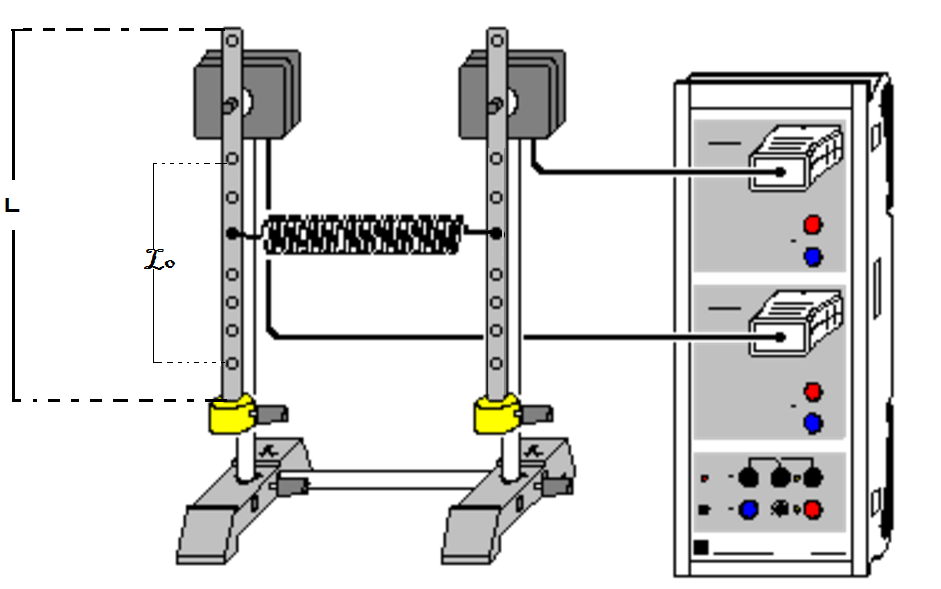
\includegraphics[width=0.80\textwidth]{img/dispositivopaco}
  \caption{Dispositivo utilizado para la practica experimental con los pendulos.}
      \label{fig:dispositivo}
\end{figure}
\begin{figure}[H]
  \centering
     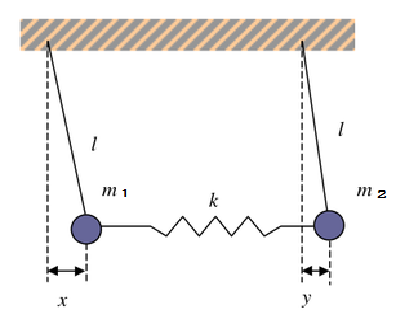
\includegraphics[width=0.80\textwidth]{img/pendulosfase}
  \caption{Representación gráfica de los péndulos en fase.}
      \label{fig:dispositivo}
\end{figure}

%%%%Fase
\begin{table}[H]
    \begin{subtable}{.5\linewidth}
      \centering 
      %%%Tabla 1
        \begin{tabular}{@{}l|l|l|@{}}
\cmidrule(l){2-3}
\multicolumn{1}{c|}{} & \multicolumn{1}{c|}{Tiempos [s]} & \multicolumn{1}{c|}{$\epsilon=l_{0}$/L}     \\ \cmidrule(l){2-3} 
                      & T1=1.115s                        & \multirow{4}{*}{$\frac{25.5cm}{40cm}=0.638cm$} \\ \cmidrule(lr){2-2}
                      & T2=1.150s                        &                                \\ \cmidrule(lr){2-2}
                      & T3=1.080s                        &                                \\ \cmidrule(lr){2-2}
\textbf{Tprom1}   & 1.115s                            &                                \\ \cmidrule(l){2-3} 
\end{tabular}
\caption{Periodos Tomados en fase$\phi$, distancia $l_{0}=25.5cm$}
\label{fase1}
    \end{subtable}%
      %%%Tabla 2
    \begin{subtable}{.8\linewidth}
      \centering
        \begin{tabular}{@{}l|l|l|@{}}
		\cmidrule(l){2-3}
\multicolumn{1}{c|}{} & \multicolumn{1}{c|}{Tiempos [s]} & \multicolumn{1}{c|}{$\epsilon=l_{0}$/L}       \\ \cmidrule(l){2-3} 
                      & T1=1.140s                        & \multirow{4}{*}{$\frac{23cm}{40cm}=0.575cm$}  \\ \cmidrule(lr){2-2}
                      & T2=1.120s                        &                                                 \\ \cmidrule(lr){2-2}
                      & T3=1.194s                        &                                  				 \\ \cmidrule(lr){2-2}
	\textbf{Tprom2}   & 1.151s                           &               				                      \\ \cmidrule(l){2-3} 
\end{tabular}
\caption{Periodos Tomados en fase$\phi$, distancia $l_{0}=\textbf{23cm}$}
\label{fase1-2}
    \end{subtable}     
     %%%Tabla 3
    \begin{subtable}{.5\linewidth}
      \centering
        \begin{tabular}{@{}l|l|l|@{}}
\cmidrule(l){2-3}
\multicolumn{1}{c|}{} & \multicolumn{1}{c|}{Tiempos [s]} & \multicolumn{1}{c|}{$\epsilon=l_{0}$/L}     \\ \cmidrule(l){2-3} 
                      & T1=1.120s                        & \multirow{4}{*}{$\frac{20.5cm}{40cm}=0.513cm$} \\ \cmidrule(lr){2-2}
                      & T2=1.165s                        &                                \\ \cmidrule(lr){2-2}
                      & T3=1.155s                        &                                \\ \cmidrule(lr){2-2}
\textbf{Tprom3}       & 1.147s                           &                                \\ \cmidrule(l){2-3} 
\end{tabular}
\caption{Periodos Tomados en fase$\phi$, distancia $l_{0}=\textbf{20.5cm}$}
\label{fase1-3}
    \end{subtable}%
    %%%Tabla 4
    \begin{subtable}{.8\linewidth}
      \centering
        \begin{tabular}{@{}l|l|l|@{}}
		\cmidrule(l){2-3}
\multicolumn{1}{c|}{} & \multicolumn{1}{c|}{Tiempos [s]} & \multicolumn{1}{c|}{$\epsilon=l_{0}$/L}       \\ \cmidrule(l){2-3} 
                      & T1=1.154s                        & \multirow{4}{*}{$\frac{18cm}{40cm}=0.450cm$}  \\ \cmidrule(lr){2-2}
                      & T2=1.174s                        &                                                 \\ \cmidrule(lr){2-2}
                      & T3=1.219s                        &                                  				 \\ \cmidrule(lr){2-2}
	\textbf{Tprom4}   & 1.182s                            &               				                      \\ \cmidrule(l){2-3} 
\end{tabular}
\caption{Periodos Tomados en fase$\phi$, distancia $l_{0}=\textbf{18cm}$}
\label{fase1-4}
    \end{subtable} 
   %%%Tabla 5
    \begin{subtable}{.5\linewidth}
      \centering
        \begin{tabular}{@{}l|l|l|@{}}
\cmidrule(l){2-3}
\multicolumn{1}{c|}{} & \multicolumn{1}{c|}{Tiempos [s]} & \multicolumn{1}{c|}{$\epsilon=l_{0}$/L}     \\ \cmidrule(l){2-3} 
                      & T1=1.194s                        & \multirow{4}{*}{$\frac{15.5cm}{40cm}=0.388cm$} \\ \cmidrule(lr){2-2}
                      & T2=1.189s                        &                                \\ \cmidrule(lr){2-2}
                      & T3=1.174s                        &                                \\ \cmidrule(lr){2-2}
\textbf{Tprom5}   	  & 1.186s                           &                                \\ \cmidrule(l){2-3} 
\end{tabular}
\caption{Periodos Tomados en fase$\phi$, distancia $l_{0}=\textbf{15.5cm}$}
\label{fase1-5}
    \end{subtable}%
   %%%Tabla 6
    \begin{subtable}{.8\linewidth}
      \centering
        \begin{tabular}{@{}l|l|l|@{}}
		\cmidrule(l){2-3}
\multicolumn{1}{c|}{} & \multicolumn{1}{c|}{Tiempos [s]} & \multicolumn{1}{c|}{$\epsilon=l_{0}$/L}       \\ \cmidrule(l){2-3} 
                      & T1=1.184s                        & \multirow{4}{*}{$\frac{13cm}{40cm}=0.325$}  \\ \cmidrule(lr){2-2}
                      & T2=1.219s                        &                                                 \\ \cmidrule(lr){2-2}
                      & T3=1.174s                        &                                  				 \\ \cmidrule(lr){2-2}
	\textbf{Tprom6}   & 1.192s                           &               				                      \\ \cmidrule(l){2-3} 
\end{tabular}
\caption{Periodos Tomados en fase$\phi$, distancia $l_{0}=\textbf{13cm}$}
\label{fase1-6}
 \end{subtable} 
    %%%Tabla 7
   
       \centering
    \begin{subtable}{.8\linewidth}
      \centering
        \begin{tabular}{@{}l|l|l|@{}}
		\cmidrule(l){2-3}
\multicolumn{1}{c|}{} & \multicolumn{1}{c|}{Tiempos [s]} & \multicolumn{1}{c|}{$\epsilon=l_{0}$/L}       \\ \cmidrule(l){2-3} 
                      & T1=1.1795s                       & \multirow{4}{*}{$\frac{10.5cm}{40cm}=0.263$}  \\ \cmidrule(lr){2-2}
                      & T2=1.202s                        &                                                 \\ \cmidrule(lr){2-2}
                      & T3=1.169s                        &                                  				 \\ \cmidrule(lr){2-2}
	\textbf{Tprom7}   & 1.183s                           &               				                      \\ \cmidrule(l){2-3} 
\end{tabular}
\caption{Periodos Tomados en fase$\phi$, distancia $l_{0}=\textbf{10.5cm}$}
\label{fase1-7}
    \end{subtable} 
\caption{Periodos Tomados en fase$\phi$, con sus respectivas distancias $l_{0}, \textbf{Tprom: Tiempos Promedio}$.}
\label{generalfase}
\end{table}
$$\\$$
Los valores adquiridos en contra fase.
\newline
\begin{table}[H]
    \begin{subtable}{.5\linewidth}
      \centering 
      %%%Tabla 1
        \begin{tabular}{@{}l|l|l|@{}}
\cmidrule(l){2-3}
\multicolumn{1}{c|}{} & \multicolumn{1}{c|}{Tiempos [s]} & \multicolumn{1}{c|}{$\epsilon=l_{0}$/L}     \\ \cmidrule(l){2-3} 
                      & T1=0.942s                        & \multirow{4}{*}{$\frac{25.5cm}{40cm}=0.638cm$} \\ \cmidrule(lr){2-2}
                      & T2=1.001s                        &                                \\ \cmidrule(lr){2-2}
                      & T3=0.986s                        &                                \\ \cmidrule(lr){2-2}
\textbf{Tprom1}       & 0.976s                           &                                \\ \cmidrule(l){2-3} 
\end{tabular}
\caption{Periodos Tomados en contrafase$\phi$, distancia $l_{0}=25.5cm$}
\label{contrafase1}
    \end{subtable}%
      %%%Tabla 2
    \begin{subtable}{.8\linewidth}
      \centering
        \begin{tabular}{@{}l|l|l|@{}}
		\cmidrule(l){2-3}
\multicolumn{1}{c|}{} & \multicolumn{1}{c|}{Tiempos [s]} & \multicolumn{1}{c|}{$\epsilon=l_{0}$/L}       \\ \cmidrule(l){2-3} 
                      & T1=1.026s                        & \multirow{4}{*}{$\frac{23cm}{40cm}=0.575cm$}  \\ \cmidrule(lr){2-2}
                      & T2=0.942s                        &                                                 \\ \cmidrule(lr){2-2}
                      & T3=0.961s                        &                                  				 \\ \cmidrule(lr){2-2}
	\textbf{Tprom2}   & 0.976s                           &               				                      \\ \cmidrule(l){2-3} 
\end{tabular}
\caption{Periodos Tomados en contrafase$\phi$, distancia $l_{0}=\textbf{23cm}$}
\label{contrafase1-2}
    \end{subtable}     
     %%%Tabla 3
    \begin{subtable}{.5\linewidth}
      \centering
        \begin{tabular}{@{}l|l|l|@{}}
\cmidrule(l){2-3}
\multicolumn{1}{c|}{} & \multicolumn{1}{c|}{Tiempos [s]} & \multicolumn{1}{c|}{$\epsilon=l_{0}$/L}     \\ \cmidrule(l){2-3} 
                      & T1=0.981s                        & \multirow{4}{*}{$\frac{20.5cm}{40cm}=0.513cm$} \\ \cmidrule(lr){2-2}
                      & T2=0.961s                        &                                \\ \cmidrule(lr){2-2}
                      & T3=0.996s                        &                                \\ \cmidrule(lr){2-2}
\textbf{Tprom3}   & 0.979s                            &                                \\ \cmidrule(l){2-3} 
\end{tabular}
\caption{Periodos Tomados en contrafase$\phi$, distancia $l_{0}=\textbf{20.5cm}$}
\label{contrafase1-3}
    \end{subtable}%
    %%%Tabla 4
    \begin{subtable}{.8\linewidth}
      \centering
        \begin{tabular}{@{}l|l|l|@{}}
		\cmidrule(l){2-3}
\multicolumn{1}{c|}{} & \multicolumn{1}{c|}{Tiempos [s]} & \multicolumn{1}{c|}{$\epsilon=l_{0}$/L}       \\ \cmidrule(l){2-3} 
                      & T1=1.026s                        & \multirow{4}{*}{$\frac{18cm}{40cm}=0.450cm$}  \\ \cmidrule(lr){2-2}
                      & T2=0.996s                        &                                                 \\ \cmidrule(lr){2-2}
                      & T3=1.016s                        &                                  				 \\ \cmidrule(lr){2-2}
	\textbf{Tprom4}   & 1.013s                           &               				                      \\ \cmidrule(l){2-3} 
\end{tabular}
\caption{Periodos Tomados en contrafase$\phi$, distancia $l_{0}=\textbf{18cm}$}
\label{contrafase1-4}
    \end{subtable} 
   %%%Tabla 5
    \begin{subtable}{.5\linewidth}
      \centering
        \begin{tabular}{@{}l|l|l|@{}}
\cmidrule(l){2-3}
\multicolumn{1}{c|}{} & \multicolumn{1}{c|}{Tiempos [s]} & \multicolumn{1}{c|}{$\epsilon=l_{0}$/L}     \\ \cmidrule(l){2-3} 
                      & T1=1.051s                        & \multirow{4}{*}{$\frac{15.5cm}{40cm}=0.388cm$} \\ \cmidrule(lr){2-2}
                      & T2=1.036s                        &                                \\ \cmidrule(lr){2-2}
                      & T3=1.041s                        &                                \\ \cmidrule(lr){2-2}
\textbf{Tprom5}   	  & 1.043s                           &                                \\ \cmidrule(l){2-3} 
\end{tabular}
\caption{Periodos Tomados en contrafase$\phi$, distancia $l_{0}=\textbf{15.5cm}$}
\label{contrafase1-5}
    \end{subtable}%
   %%%Tabla 6
    \begin{subtable}{.8\linewidth}
      \centering
        \begin{tabular}{@{}l|l|l|@{}}
		\cmidrule(l){2-3}
\multicolumn{1}{c|}{} & \multicolumn{1}{c|}{Tiempos [s]} & \multicolumn{1}{c|}{$\epsilon=l_{0}$/L}       \\ \cmidrule(l){2-3} 
                      & T1=1.080s                        & \multirow{4}{*}{$\frac{13cm}{40cm}=0.325$}  \\ \cmidrule(lr){2-2}
                      & T2=1.090s                        &                                                 \\ \cmidrule(lr){2-2}
                      & T3=1.075s                        &                                  				 \\ \cmidrule(lr){2-2}
	\textbf{Tprom6}   & 1.082s                          &               				                      \\ \cmidrule(l){2-3} 
\end{tabular}
\caption{Periodos Tomados en contrafase$\phi$, distancia $l_{0}=\textbf{13cm}$}
\label{contrafase1-6}
 \end{subtable} 
    %%%Tabla 7
       \centering
    \begin{subtable}{.8\linewidth}
      \centering
        \begin{tabular}{@{}l|l|l|@{}}
		\cmidrule(l){2-3}
\multicolumn{1}{c|}{} & \multicolumn{1}{c|}{Tiempos [s]} & \multicolumn{1}{c|}{$\epsilon=l_{0}$/L}       \\ \cmidrule(l){2-3} 
                      & T1=1.0905s                       & \multirow{4}{*}{$\frac{10.5cm}{40cm}=0.263$}  \\ \cmidrule(lr){2-2}
                      & T2=1.125s                        &                                                 \\ \cmidrule(lr){2-2}
                      & T3=1.125s                        &                                  				 \\ \cmidrule(lr){2-2}
	\textbf{Tprom7}   & 1.113s                           &               				                      \\ \cmidrule(l){2-3} 
\end{tabular}
\caption{Periodos Tomados en contrafase$\phi$, distancia $l_{0}=\textbf{10.5cm}$}
\label{contrafase1-7}
    \end{subtable} 
\caption{Periodos Tomados en contrafase$\phi$, con sus respectivas distancias $l_{0}, \textbf{Tprom: Tiempos Promedio}$.}
\label{generalcontrafase}
\end{table}
$\\$
$\\$
$\\$
$\\$
El periodo para péndulos en fase$\phi$(\textit{21 oscilaciones}) es:
$$t=\sum _{ i=1 }^{ 7 }{ { Tprom }_{ i } } =24,470$$
$$\frac{t}{n}=\frac{24,470}{21}=1,165$$
$${ T }_{ fase }=1,165s$$
El periodo para péndulos en contra fase$\phi$ (\textit{21 oscilaciones}) es:
$$t=\sum _{ i=1 }^{ 7 }{ { Tprom }_{ i } } =21,547$$
$$\\$$
$$\frac{t}{n}=\frac{21,547}{21}=1,026$$
$$\\$$
$${ T }_{ Contrafase }=1,026s$$
\newline
\section{Análisis}
\subsection{(Pregunta 2.7.1)}
Con los datos experimentales hallados en los numerales 4, 5 y 6 obtenga ${ \omega  }_{ 1 }$ y ${ \omega  }_{ 2 }$ 
con sus respectivas incertidumbres.\\
considerando que por definición tenemos :\newline
\begin{equation}
{ \omega  }_{ 1 }=\frac { 2*\Pi  }{ { T }_{ fase } }
\end{equation} 
\begin{equation}
{ \omega  }_{ 2 }=\frac { 2*\Pi  }{ { T }_{ contrafase } } 
\end{equation}

sustituyendo en las ecuaciones anteriores, los valores de ${ T }_{ fase }  , { T }_{ contrafase } $
$${ \omega  }_{ 1 }=\frac { 2*\Pi  }{1,165s} =5.393rad/s\\$$
hallando ${ \omega  }_{ 2 }$ con periodo ${ T }_{ contrafase=1.026s}$ :
$${ \omega  }_{ 2 }=\frac { 2*\Pi  }{1,026s} =\textbf{6.124}rad/s\\$$
comparando contra :
$${ \omega  }_{ 2 }^{ 2 }=\frac { g }{ L } +2{ \epsilon  }^{ 2 }\frac { k }{ m } $$\\
$${ \omega  }_{ 2 }=\sqrt { \frac { g }{ L } +2{ \epsilon  }^{ 2 }\frac { k }{ m }  } $$\\
$${ \omega  }_{ 2 }=\sqrt { \frac { 9.8 }{ 0.4m } +2{ \frac { 25.5 }{ 40 }  }^{ 2 }\frac { 2,9754 }{ 100.9 }  }$$\\
$${ \omega  }_{ 2 }=\quad \textbf{5.78}rad/s$$

Si tomamos los 7 tiempos promedios, y  promediamos estos tendremos un Periodo de las primeras 21 oscilaciones, \\
$T=\textbf{1.652s}$ Para un periodo total de fase.
\newline
\begin{table}[H]
\centering
\begin{tabular}{|l|l|}
\hline
${ \omega  }_{ 1 }$ & ${ \omega  }_{ 2 }$ \\ \hline
5,635  & 6,435     \\ \hline
5,457   & 6,416  \\ \hline
5,480   & 6,416  \\ \hline
5,393   & 6,205  \\ \hline
5,299   & 6,026  \\ \hline
5,270   & 5,809  \\ \hline
5,310   & 5,644  \\ \hline
\end{tabular}
\caption{Tabla de datos obtenidos al aplicar las ecuaciones, considerando cada tiempo promedio}
\label{general}
\end{table}
\subsection{(Pregunta 2.7.2) }
Con los valores obtenidos, construya una gráfica de ${ \omega  }_{ 2 }^{ 2 }$  y ${\epsilon}^{ 2 }$
$\\$
$\\$
Utilizando los siguientes valores se construyo la siguiente grafica
\begin{table}[H]
\centering
\begin{tabular}{|l|l|}
\hline
${ \omega  }_{ 2 }^{ 2 }$ & ${ \epsilon  }^{ 2 }$ \\ \hline
0,407&	   48,469\\ \hline
0,331&      42,550    \\ \hline
0,263   &   38,840    \\ \hline
0,203   &	35,555    \\ \hline
0,151   &	32,698    \\ \hline
0,106   &	30,267    \\ \hline
0,069   &	28,262    \\ \hline
 \end{tabular}
\caption{Datos para graficar ${ \omega  }_{ 2 }^{ 2 }$  vs ${ \epsilon  }^{ 2 }$.}
\label{grafical}
\end{table}
\begin{figure}[H]
 \centering
   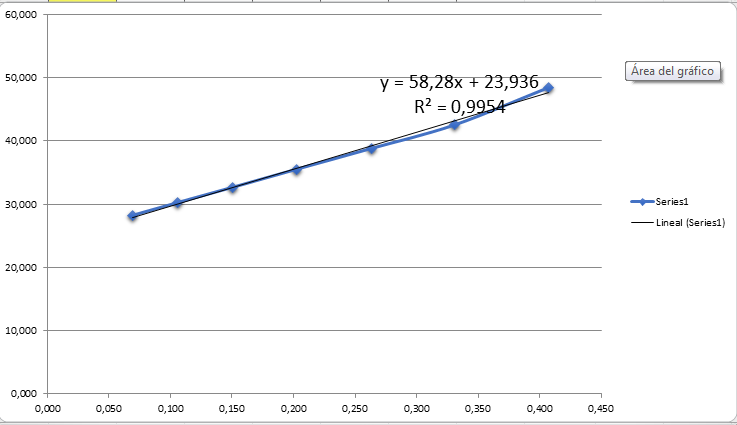
\includegraphics[width=0.9\textwidth]{img/grafica}
 \caption{Grafica ${ \omega  }_{ 2 }^{ 2 }$  vs ${ \epsilon  }^{ 2 }$}
    \label{fig:modelo}
\end{figure}


\subsection{(Pregunta 2.7.3) }
Determine la ecuación experimental a partir de su gráfico y por comparación con la ecuación (\textbf{2.8}):determine los valores de $g$ y $k$ \newline
La ecuación \textbf{(2.8)} esta dada por la siguiente expresión:
\begin{equation} y=Ax+B \end{equation}
hallando la ecuación experimental a partir del gráfico obtenemos

\begin{equation}
 y=58,28x+23,936\quad
\end{equation}
\textbf{R}=0,9954 en la grafica es nuestro coeficiente de determinación indica que la representación gráfica de la Figure 1 es muy precisa. Si utilizamos los coeficientes \textbf{A, B} es posible hallar la gravedad experimental \textbf{g} y la constante elástica \textbf{k}.
\newline
Para obtener la gravedad experimental sabemos que :
\begin{equation}
g=B*L
\end{equation}
$$g=23,936{ s }^{ -2 }*0,40m$$
que nos da como resultado:
$$g=9.574\frac { m }{ { s }^{ 2 } } $$
Para obtener la constante elástica \textbf{k} por definición:
\begin{equation}
 K=\frac { AM }{ 2 }
\end{equation}
reemplazando los coeficientes correspondientes:
$$k =\frac { 58,28*0.1kg }{ 2 }=2.914$$


\subsection{(Pregunta 2.7.4) }
Compare el valor de g con el valor aceptado. Encuentre su porcentaje de error. Si se conoce el valor teórico para la constante k, halle también su porcentaje de error.
Porcentaje de error k.
\newline
Para desarrollar este punto utilizaremos la siguiente expresion para determinar los errores:
\begin{equation}
    \% Error = \frac{|Valor \ esperado-Valor \ experimental|}{Valor esperado}*100\%
\end{equation}
\newline
Determinando el error porcentual del valor hallado para la gravedad \textbf{\textit{g}} tenemos:
$$\% Error  \textbf{g}= \frac{|9.8-9.574|}{9.8}*100\%=2.3\% $$
\newline
Determinando el error porcentual para el valor hallado del coeficiente \textbf{\textit{k}} tenemos:
$$
    \% Error \textbf{k} = \frac{|2.9754-2.914|}{2.9754}*100\%=2.06\%    
$$

\subsubsection{Análisis de Incertidumbre,para  g, k }
De definición matemática:
\begin{equation}
  \upsilon _{A} = \sqrt{ \frac{ {\sum_{i=1}^{n} (x_{i}- \overline{x})^{2}} }{n(n-1)}  }
\end{equation}
\\
Para medidas con instrumentos Análogos:
\begin{equation}
  \upsilon _{B1} =\frac{Resolucion}{\sqrt{3}}
\end{equation}
Para medidas con instrumentos Digitales:
\begin{equation}
  \upsilon _{B2} =\frac{Resolucion}{2\sqrt{3}}
\end{equation}
La Incertidumbre combinada esta determinada por la siguiente expresión :
\begin{equation}
    U_{C} = \sqrt{(\upsilon _{A})^2+(\upsilon _{B1})^2+(\upsilon _{B2})^2}
\end{equation}
\subsubsection{Análisis de Incertidumbre, Constante \textbf{g} }
\begin{equation}
\frac{\partial g}{\partial B} =L \qquad \frac{\partial g}{\partial L} = B
\end{equation}

Respecto de $L$
$${ Ib }^{ 2 }=\frac { 0.400m**0.00100 }{ \sqrt { 3 }  } $$
\\
$${ Ib }^{ 2 }=2.31*{10}^{ -4 }m$$
$$\delta L=|2.31*{10}^{ -4 }m|= 2.31*{10}^{ -4 }m$$

Respecto de $B$\\
$$\delta B=|0.01382{s}^{-2}|= 0.01382{s}^{-2}$$
\textbf{Incertidumbre Combinada para g}

$$Incertidumbre=\left[ 23.936* 2.31*{ 10 }^{ -4 }m \right] +\left[ 0.40m*0.01382\right]$$
$$Incertidumbre=11.057*{ 10 }^{ -3 }$$
El valor de la constante g obtenido fue de :
$$g=(9.574\pm \quad 11.057*{ 10 }^{ -3 })N/m$$

\subsubsection{Análisis de Incertidumbre, Constante \textbf{k} }
\begin{equation}
\frac{\partial k}{\partial A} = \frac{M}{2} \qquad \frac{\partial k}{\partial M} = \frac{A}{2} 
\end{equation}

Respecto de $A$
$${ Ib }^{ 2 }=\frac { 58.28{ s }^{ -2 }*0.001 }{ \sqrt { 3 }  } $$
$$
{ Ib }^{ 2 }=0,03365{ s }^{ -2 }$$
$$\delta A=|0,03365{ s }^{ -2 }|=0,03365{ s }^{ -2 }$$
Con Respecto de $M$
$${ Ib }^{ 2 }=\frac { 0.0497kg*0.001 }{ \sqrt { 3 }  } $$
$$
{ Ib }^{ 2 }=2.86*{10}^{ -5 }kg$$
$$\delta M=|2.86*{10}^{ -5 }kg|=2.86*{10}^{ -5 }kg$$
\textbf{Incertidumbre Combinada para K}
$$Incertidumbre=\left[ \frac { 0.1 }{ 2 } *2.86*{ 10 }^{ -5 } \right] kg+\left[ \frac { 58.28 }{ 2 } *0.03364\right]$$
\\$$
Incertidumbre=0.971
$$
El valor de la constante K obtenido fue de :
$$K=(2.914\pm 0.971)N/m$$

Se puede observar que los valores obtenidos experimentalmente comparados con los puntos teóricos tienen aproximaciones muy cercanas, por lo que podemos afirmar que el procedimiento realizado para obtener los coeficientes \textbf{\textit{k, g}} es el correcto. 

\section{Errores Considerados}
Los errores considerados para esta practica  según los instrumentos fueron :
\begin{itemize}
	\item	Error en la regla = 0.001 m
	\item	Error del observador = 0.001m
	\item	Error en la balanza = 0.1 gr.
	\item	Error de la calibración del cronometro = 0.01seg
	\item	Error para la medición de la K del resorte
	\item	Existe un error entre el tiempo en que se sueltan los péndulos y el momento en que comienza a contar el cronómetro; este error no tiene un valor exacto.
\end{itemize}

Si realizamos la sumatoria de los errores, nuestro error estimado total es :
$$\\ Etotal=\sqrt { { 0.001gr }^{ 2 }+{ 0.001gr }^{ 2 }+{ 0.1gr }^{ 2 }+{ 0.01gr }^{ 2 } } =\textbf{0.1005087}$$
\subsection{Conclusiones }
De la practica experimental, y la teoría conocida podemos concluir:
\begin{itemize}
	\item Los péndulos acoplados gozan de una transmisión de la energía, en los puntos extremos del periodo, en el sistema.
    \item Se pudo observar que en esta practica de péndulos acoplados hay varios principios físicos, como la transferencia , conservación y la transformación de energía.
    \item Se identificaron y determinaron las frecuencias propias de oscilación para un sistema de péndulos acoplados con dos grados de libertad.
	\item Se determinó el valor de la aceleración de la gravedad. 
\end{itemize}
\section{Bibliografia}
$[1]$ Raymond A. Serway Physics for Scientists and Engineers with Modern Physics. 
$\\$
$[2]$ Sears and Zemansky's University Physics.
$\\$
$[3]$ Resonant Couple Pendulums, www.exploratorium.edu
$\\$
$[4]$ Martín del Campo, Javier Miranda. “Evaluación de la incertidumbre en datos experimentales”. Disponible en Google Drive utp.edu.co 
\end{document}